% ------------------------------------------------------------------------------
% Resultados e discussão
% ------------------------------------------------------------------------------

\chapter{Resultados e discussão}
\label{chap_resultados}

Este capítulo apresenta os resultados em quatro etapas.
A \autoref{sec_execucao_financeira} descreve a execução financeira do Pé-de-Meia em 2024.
A \autoref{sec_series_descritivas} apresenta a evolução descritiva dos indicadores educacionais por rede.
A \autoref{sec_estimativas_did} reporta as estimativas de Diferenças em Diferenças e os testes de pré-tendência.
Por fim, a \autoref{sec_discussao} discute os resultados à luz da literatura e das limitações do delineamento.
Em todas as tabelas e figuras, as médias por rede correspondem à média simples das 27 UFs, coerente com a ponderação implícita dos modelos em painel.

% ------------------------------------------------------------------------------
\section{Execução financeira do Pé-de-Meia em 2024}
\label{sec_execucao_financeira}

A \autoref{tab_execucao_mensal} apresenta a execução mensal nacional do programa no exercício de 2024.
O montante transferido cresce ao longo do ano, passando de R\$ 483,3 milhões na primeira folha para valores próximos de R\$ 686 milhões nos meses finais, em razão da incorporação progressiva de novos beneficiários.
O exercício totalizou R\$ 5.587.440.225,00 em 27.892.528 parcelas.

\begin{table}[!htb]
    \centering
    \caption{Execução mensal nacional do Pé-de-Meia no exercício de 2024}
    \label{tab_execucao_mensal}
    \small
    \begin{tabularx}{\textwidth}{cXrr}
        \toprule
        \textbf{Folha} & \textbf{Observação operacional} & \textbf{Valor (R\$)} & \textbf{Parcelas} \\
        \midrule
        03/2024 & 1º lote de matrícula (versão retificada) & 483.250.400,00 & 2.416.252 \\
        04/2024 & 1ª parcela de frequência e matrícula complementar & 552.561.000,00 & 2.762.805 \\
        05/2024 & 2ª parcela de frequência e matrícula complementar & 549.488.000,00 & 2.747.440 \\
        06/2024 & 3ª parcela de frequência e matrícula complementar & 659.172.000,00 & 3.295.860 \\
        08/2024 & Retomada pós-recesso e expansão do público & 630.427.600,00 & 3.152.138 \\
        09/2024 & Parcela regular & 656.487.400,00 & 3.282.437 \\
        10/2024 & Parcela regular & 686.305.175,00 & 3.418.224 \\
        11/2024 & Parcela regular & 683.902.550,00 & 3.404.749 \\
        12/2024 & Última folha do exercício & 685.846.100,00 & 3.412.623 \\
        \midrule
        \multicolumn{2}{l}{\textbf{Total do exercício de 2024 (9 folhas)}} & \textbf{5.587.440.225,00} & \textbf{27.892.528} \\
        \bottomrule
    \end{tabularx}
    \fonte{Elaborada pelo autor (2026) com dados de \citeonline{CGU2026PeDeMeia}. Não há folha em julho, em razão do recesso escolar.}
\end{table}

Ao exercício de 2024 somam-se os depósitos de conclusão (3.037.316 parcelas; R\$ 3,04 bilhões) e de Enem (450.679 parcelas; R\$ 90,1 milhões) referentes ao ano letivo de 2024, pagos na folha de fevereiro de 2025.
O custo do ciclo letivo de 2024 contabilizado até fevereiro de 2025 é, portanto, de R\$ 8.714.892.025,00, valor que deve ser interpretado como um \textit{piso}, pois a folha de março de 2025 ainda contém pagamentos retroativos de conclusão do ano letivo de 2024 (ao menos 111.734 parcelas nas 16 UFs disponíveis no arquivo parcial analisado).
Dividido pelas 4.008.269 parcelas de matrícula (\textit{proxy} de estudantes beneficiários), esse piso corresponde a R\$ 2.174,23 por estudante.

A \autoref{fig_repasses_uf} apresenta a distribuição dos repasses de 2024 por pessoa cadastrada no CadÚnico em cada UF.
Observa-se um claro gradiente regional: as UFs do Nordeste e do Norte concentram os maiores valores relativos, liderados por Maranhão (R\$ 79,54) e Pará (R\$ 78,93), enquanto as UFs do Sul e do Sudeste ocupam as últimas posições, com Rio Grande do Sul (R\$ 38,94) e Paraná (R\$ 41,00).
A razão nacional agregada é de R\$ 58,61 por pessoa cadastrada.
Esse padrão é compatível com a maior proporção de jovens de famílias de baixa renda matriculados no ensino médio público nessas regiões.
Alagoas, com R\$ 72,86 por pessoa cadastrada, situa-se na quarta posição nacional.
A tabela completa por UF encontra-se no \autoref{chap_apendice_uf}.

\begin{figure}[!htb]
    \centering
    \caption{Repasses do Pé-de-Meia por pessoa cadastrada no CadÚnico, por UF (exercício de 2024)}
    \label{fig_repasses_uf}
    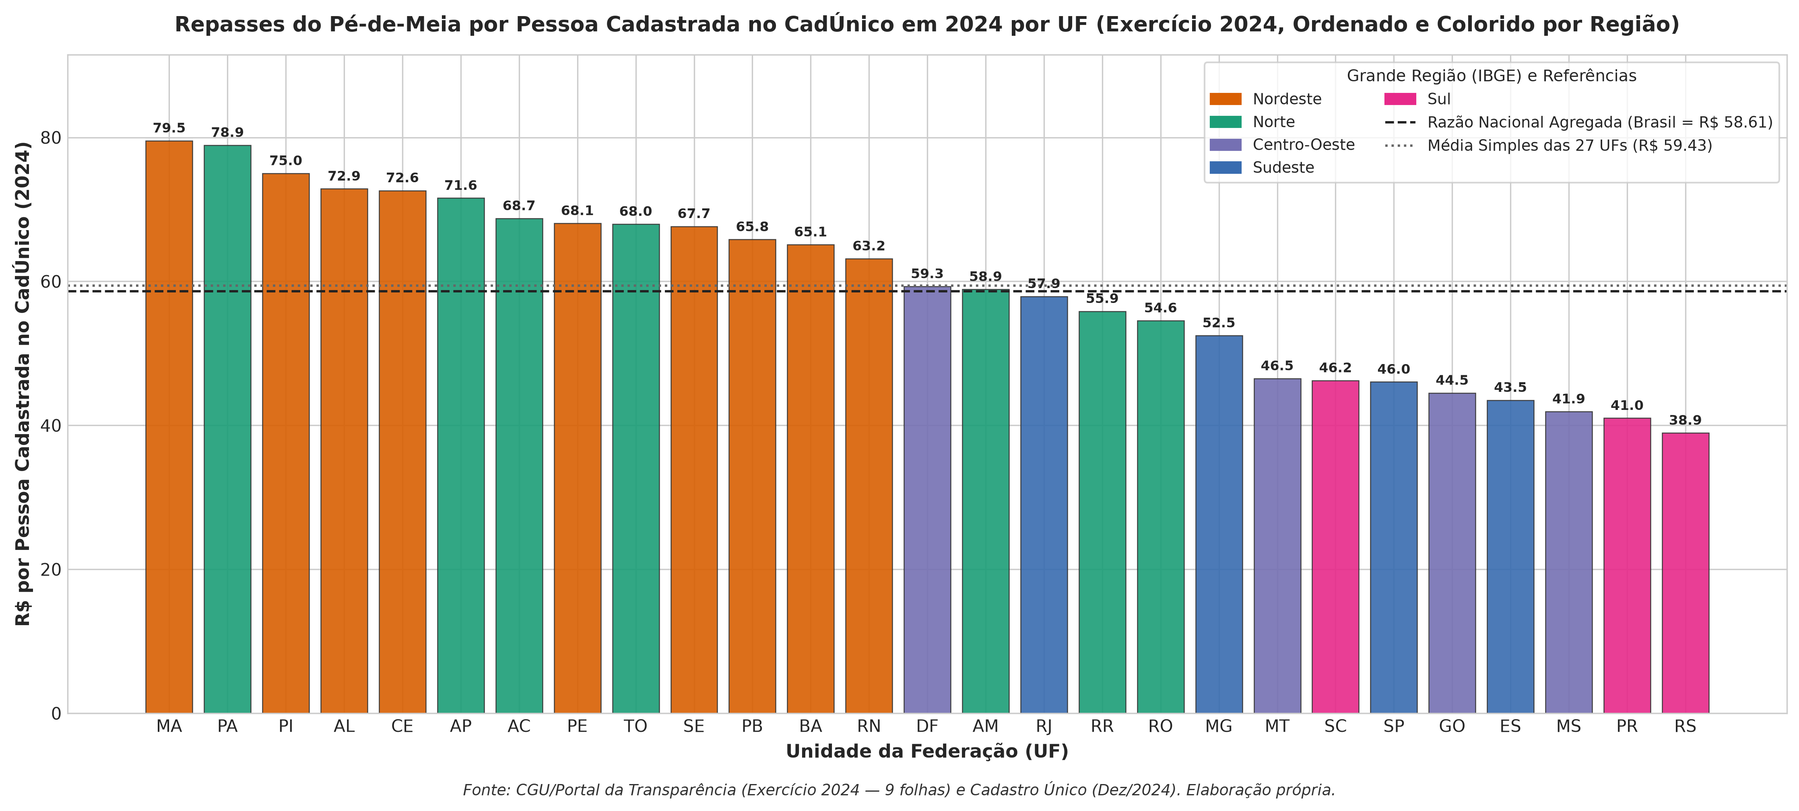
\includegraphics[width=\textwidth]{figuras/grafico_repasses_pedemeia_uf_nacional}
    \fonte{Elaborada pelo autor (2026) com dados de \citeonline{CGU2026PeDeMeia} e \citeonline{Alagoas2026CadUnico}.}
\end{figure}

O custo por estudante (\textit{proxy}) no exercício de 2024 foi de R\$ 1.393,98 no agregado nacional, variando de R\$ 1.133,91 no Amazonas a R\$ 1.566,76 no Pará.
Na folha de fevereiro de 2025, a razão entre parcelas de conclusão e total de pagamentos de 2024 foi de 10,89\% no agregado nacional, mas atipicamente baixa no Amapá (4,03\%) e em Santa Catarina (2,84\%).
No caso do Amapá, verificou-se nos microdados de março de 2025 que outras 10.797 parcelas de conclusão do ano letivo de 2024 foram pagas nessa folha, o que comprova o pagamento defasado.
Para Santa Catarina, cuja UF não consta no arquivo parcial disponível, formula-se a mesma hipótese.
Por essa razão, as comparações financeiras entre UFs utilizam exclusivamente o exercício fechado de 2024.

% ------------------------------------------------------------------------------
\section{Evolução descritiva dos indicadores educacionais}
\label{sec_series_descritivas}

\subsection{Taxas de rendimento escolar}
\label{subsec_resultados_rendimento}

A \autoref{tab_taxas_rendimento} e a \autoref{fig_taxas_rendimento} apresentam a evolução das taxas de rendimento do ensino médio por rede entre 2022 e 2025.
A taxa média de abandono da rede estadual caiu de 7,09\% em 2022 para 2,51\% em 2025, enquanto na rede privada passou de 0,88\% para 0,36\%.
Em consequência, o hiato de abandono entre as redes reduziu-se de 6,21 para 2,14 pontos percentuais.

Contudo, a maior parte dessa convergência ocorreu entre 2022 e 2023, \textit{antes} da implantação do programa: nesse intervalo, o abandono estadual recuou 3,08 p.p., contra apenas 0,11 p.p. na rede privada.
Esse movimento é compatível com a recuperação pós-pandemia e antecipa o principal desafio de identificação discutido na \autoref{sec_estimativas_did}.

\begin{table}[!htb]
    \centering
    \caption{Taxas de rendimento do ensino médio por rede (média simples das 27 UFs, em \%)}
    \label{tab_taxas_rendimento}
    \small
    \begin{tabular}{lccccccc}
        \toprule
        & \multicolumn{2}{c}{\textbf{Aprovação}} & \multicolumn{2}{c}{\textbf{Reprovação}} & \multicolumn{2}{c}{\textbf{Abandono}} & \textbf{Hiato de} \\
        \cmidrule(lr){2-3} \cmidrule(lr){4-5} \cmidrule(lr){6-7}
        \textbf{Ano} & Estadual & Privada & Estadual & Privada & Estadual & Privada & \textbf{abandono} \\
        \midrule
        2022 & 84,12 & 96,62 & 8,79 & 2,50 & 7,09 & 0,88 & 6,21 \\
        2023 & 89,78 & 96,85 & 6,21 & 2,39 & 4,01 & 0,77 & 3,24 \\
        2024 & 90,07 & 97,26 & 6,20 & 2,19 & 3,73 & 0,55 & 3,18 \\
        2025 & 93,80 & 97,61 & 3,70 & 2,02 & 2,51 & 0,36 & 2,14 \\
        \midrule
        $\Delta$ 2022--2023 (pré) & $+5{,}66$ & $+0{,}23$ & $-2{,}58$ & $-0{,}12$ & $-3{,}08$ & $-0{,}11$ & $-2{,}97$ \\
        $\Delta$ pós $-$ pré\textsuperscript{a} & $+4{,}99$ & $+0{,}70$ & $-2{,}55$ & $-0{,}34$ & $-2{,}43$ & $-0{,}37$ & $-2{,}07$ \\
        \bottomrule
    \end{tabular}
    \fonte{Elaborada pelo autor (2026) com dados de \citeonline{INEP2026Rendimento}. \textsuperscript{a}Média de 2024--2025 menos média de 2022--2023. Hiato = Estadual $-$ Privada, em p.p.}
\end{table}

\begin{figure}[!htb]
    \centering
    \caption{Taxas médias de abandono e de aprovação no ensino médio por rede (2022--2025)}
    \label{fig_taxas_rendimento}
    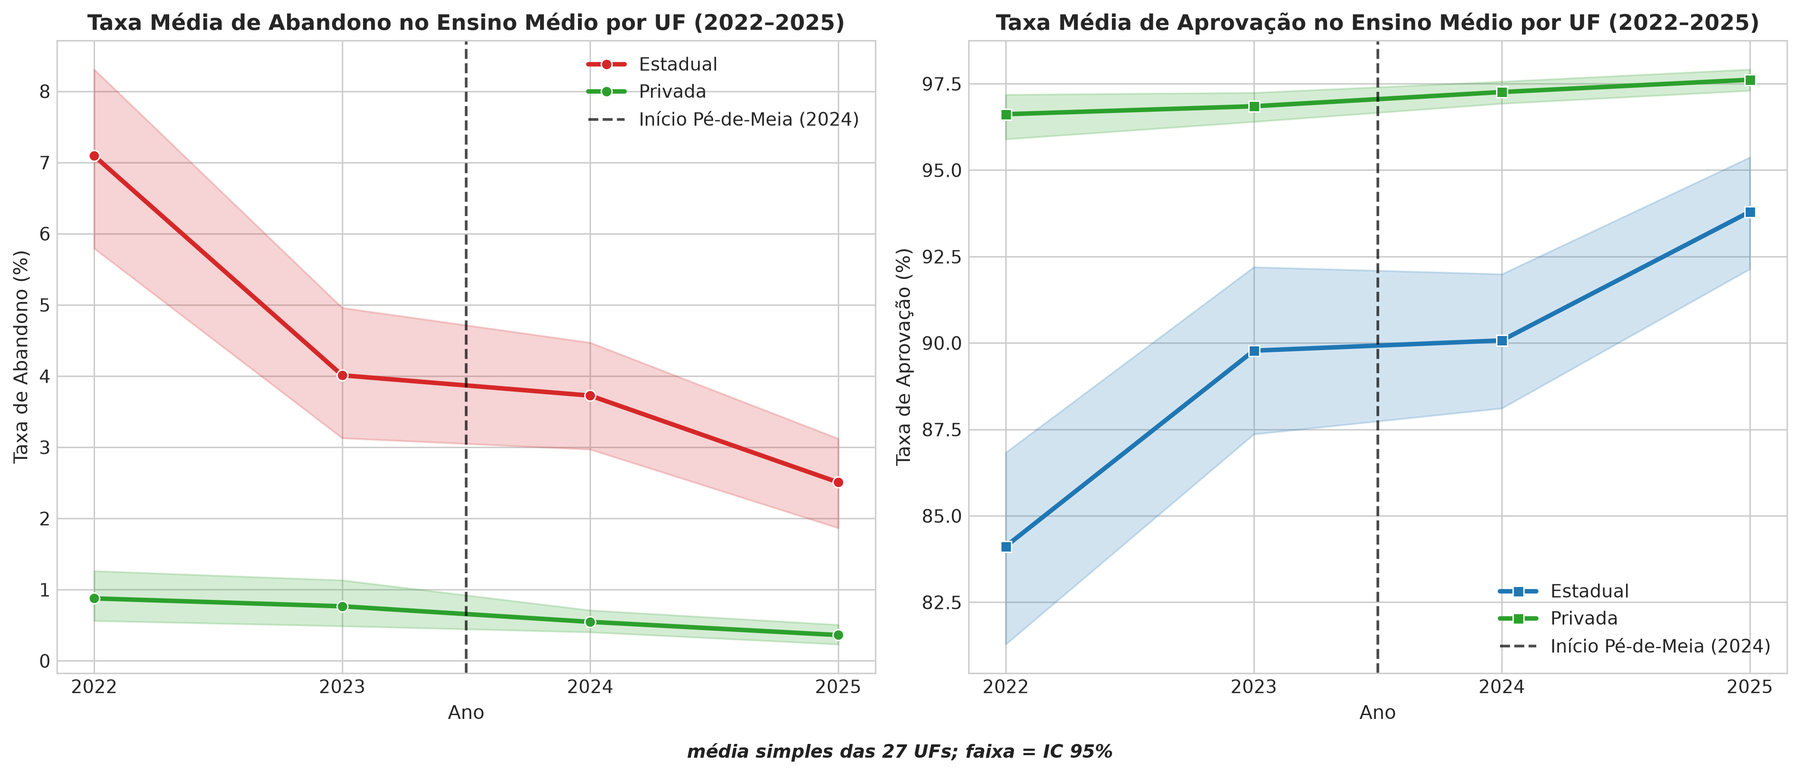
\includegraphics[width=\textwidth]{figuras/grafico_taxas_rendimento_2025}
    \fonte{Elaborada pelo autor (2026) com dados de \citeonline{INEP2026Rendimento}. Média simples das 27 UFs; a faixa sombreada representa o intervalo de confiança de 95\%.}
\end{figure}

Observa-se ainda que a rede privada já operava, em 2022, próxima dos limites da escala percentual, com aprovação de 96,62\% e abandono de 0,88\%.
Formula-se, assim, a hipótese de \textit{compressão assintótica}: como a rede privada dispõe de pouca margem para melhorar, qualquer recuperação expressiva da rede estadual se traduz mecanicamente em convergência entre as redes, independentemente da existência de uma intervenção específica.

\subsection{Desempenho no SAEB e IDEB}
\label{subsec_resultados_ideb}

A \autoref{fig_ideb_matematica} apresenta a evolução da nota do SAEB em Matemática e do IDEB por rede.
Entre 2019 e 2021, ambas as redes sofreram perdas de proficiência associadas à pandemia, mais acentuadas na rede privada (de 331,17 para 316,58 pontos em Matemática) do que na estadual (de 266,21 para 261,11 pontos).
Essa assimetria já produz uma aproximação entre as redes antes do programa.

\begin{figure}[!htb]
    \centering
    \caption{Evolução da nota do SAEB em Matemática e do IDEB do ensino médio por rede (2019--2025)}
    \label{fig_ideb_matematica}
    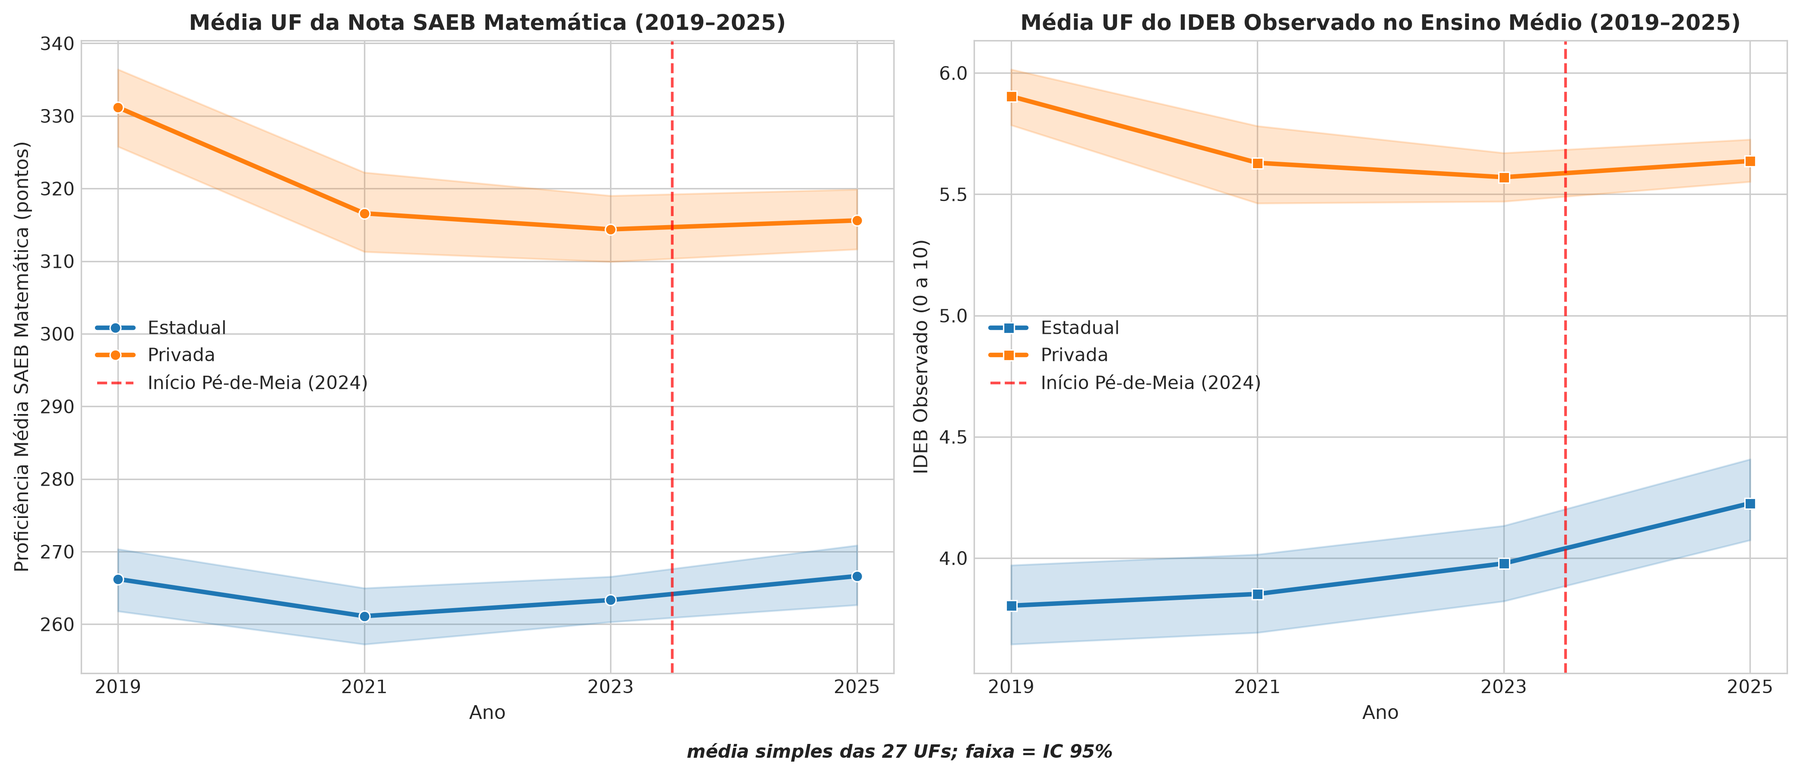
\includegraphics[width=\textwidth]{figuras/grafico_ideb_matematica_evolucao}
    \fonte{Elaborada pelo autor (2026) com dados de \citeonline{INEP2026IDEB}. Média simples das 27 UFs; a faixa sombreada representa o intervalo de confiança de 95\%.}
\end{figure}

A \autoref{tab_decomposicao_ideb} detalha a evolução do IDEB e de seus componentes.
Entre 2023 e 2025, o IDEB estadual avançou 0,2481 ponto, contra 0,0667 na rede privada.
Pela decomposição da \autoref{eq_decomposicao}, a contribuição do fluxo escolar na rede estadual é de aproximadamente $\bar{N}\,\Delta P \approx 4{,}44 \times 0{,}0377 = 0{,}167$ ponto, ou 67,5\% do ganho total.
Assim, cerca de dois terços do avanço do IDEB estadual no período decorrem da melhoria das taxas de aprovação, e não da proficiência.

\begin{table}[!htb]
    \centering
    \caption{Evolução do SAEB, dos componentes $N$ e $P$ e do IDEB do ensino médio por rede (média simples das 27 UFs)}
    \label{tab_decomposicao_ideb}
    \small
    \begin{tabular}{llrrrrr}
        \toprule
        \textbf{Indicador} & \textbf{Rede} & \textbf{2019} & \textbf{2021} & \textbf{2023} & \textbf{2025} & \textbf{$\Delta$ 2023--2025} \\
        \midrule
        \multirow{2}{*}{SAEB Matemática} & Estadual & 266,21 & 261,11 & 263,33 & 266,63 & $+3{,}30$ \\
                                          & Privada  & 331,17 & 316,58 & 314,38 & 315,61 & $+1{,}23$ \\
        \addlinespace
        \multirow{2}{*}{SAEB Língua Portuguesa} & Estadual & 269,09 & 267,53 & 267,83 & 270,71 & $+2{,}88$ \\
                                                 & Privada  & 319,97 & 310,75 & 311,26 & 310,68 & $-0{,}58$ \\
        \addlinespace
        \multirow{2}{*}{Nota padronizada ($N$)} & Estadual & 4,4567 & 4,3618 & 4,3974 & 4,4869 & $+0{,}0895$ \\
                                                 & Privada  & 6,1307 & 5,7879 & 5,7646 & 5,7731 & $+0{,}0085$ \\
        \addlinespace
        \multirow{2}{*}{Indicador de rendimento ($P$)} & Estadual & 0,8503 & 0,8828 & 0,9037 & 0,9414 & $+0{,}0377$ \\
                                                        & Privada  & 0,9628 & 0,9721 & 0,9663 & 0,9778 & $+0{,}0116$ \\
        \addlinespace
        \multirow{2}{*}{IDEB ($N \times P$)} & Estadual & 3,8037 & 3,8519 & 3,9778 & 4,2259 & $+0{,}2481$ \\
                                              & Privada  & 5,9037 & 5,6296 & 5,5704 & 5,6370 & $+0{,}0667$ \\
        \bottomrule
    \end{tabular}
    \fonte{Elaborada pelo autor (2026) com dados de \citeonline{INEP2026IDEB}.}
\end{table}

% ------------------------------------------------------------------------------
\section{Estimativas de Diferenças em Diferenças}
\label{sec_estimativas_did}

\subsection{Associações no período pós-programa}
\label{subsec_did_pos}

A \autoref{tab_did_pos} reporta os 13 coeficientes DiD estimados pela \autoref{eq_did}.
Nas taxas anuais de rendimento, a rede estadual apresentou, em relação à privada, redução diferencial de 2,07 p.p. no abandono, aumento de 4,28 p.p. na aprovação e redução de 2,21 p.p. na reprovação no período 2024--2025, todos significativos inclusive após a correção de Bonferroni.

No painel bienal completo (2019--2025), todos os indicadores do SAEB e do IDEB apresentam coeficientes positivos e significativos.
Entretanto, essas estimativas comparam o período pós-programa com uma média que inclui 2019, ano anterior às perdas pandêmicas assimétricas descritas na \autoref{subsec_resultados_ideb}, e estão, portanto, contaminadas pela divergência pré-existente entre as redes.

Na janela imediata (2023 \textit{versus} 2025), que isola a transição em torno da implantação, as notas do SAEB em Matemática ($p = 0{,}3814$) e em Língua Portuguesa ($p = 0{,}0817$) e a nota padronizada $N$ ($p = 0{,}1830$) deixam de ser significativas ao nível de 5\%.
O indicador de rendimento $P$ apresenta significância limítrofe ($p = 0{,}0505$), e o IDEB, coeficiente de $+0{,}1815$ ($p = 0{,}0115$), valor que não supera o limiar de Bonferroni para os cinco desfechos da janela ($\alpha_{\text{Bonf}} = 0{,}0100$).
Esse resultado deve, portanto, ser considerado apenas \textit{sugestivo} e interpretado em conjunto com seus componentes: o avanço do IDEB reflete sobretudo o fluxo escolar ($P$), sem ganho estatisticamente significativo de proficiência ($N$).

\begin{table}[!htb]
    \centering
    \caption{Estimativas de Diferenças em Diferenças no período pós-programa (efeitos fixos de UF $\times$ rede e de ano)}
    \label{tab_did_pos}
    \small
    \begin{tabular}{llcrrrr}
        \toprule
        \textbf{Desfecho} & \textbf{Janela} & \textbf{$n$} & \textbf{$\hat{\beta}$} & \textbf{EP} & \textbf{$t$} & \textbf{Valor-$p$} \\
        \midrule
        \multicolumn{7}{l}{\textit{Painel A -- Taxas anuais de rendimento (p.p.)}} \\
        Abandono   & 2022--2025 & 216 & $-2{,}0685$ & 0,3477 & $-5{,}949$ & $<0{,}0001$\textsuperscript{\dag} \\
        Aprovação  & 2022--2025 & 216 & $+4{,}2833$ & 0,7980 & $+5{,}368$ & $<0{,}0001$\textsuperscript{\dag} \\
        Reprovação & 2022--2025 & 216 & $-2{,}2148$ & 0,5958 & $-3{,}718$ & $0{,}0010$\textsuperscript{\dag} \\
        \addlinespace
        \multicolumn{7}{l}{\textit{Painel B -- Painel bienal completo}} \\
        SAEB Matemática (pts)        & 2019--2025 & 216 & $+8{,}1802$ & 2,0593 & $+3{,}972$ & $0{,}0005$\textsuperscript{\dag} \\
        SAEB Língua Portuguesa (pts) & 2019--2025 & 216 & $+5{,}8777$ & 1,7242 & $+3{,}409$ & $0{,}0021$\textsuperscript{\dag} \\
        Nota padronizada ($N$)       & 2019--2025 & 216 & $+0{,}2029$ & 0,0530 & $+3{,}825$ & $0{,}0007$\textsuperscript{\dag} \\
        Indicador de rendimento ($P$) & 2019--2025 & 216 & $+0{,}0517$ & 0,0112 & $+4{,}623$ & $0{,}0001$\textsuperscript{\dag} \\
        IDEB ($N \times P$)          & 2019--2025 & 216 & $+0{,}4123$ & 0,0731 & $+5{,}639$ & $<0{,}0001$\textsuperscript{\dag} \\
        \addlinespace
        \multicolumn{7}{l}{\textit{Painel C -- Janela imediata}} \\
        SAEB Matemática (pts)        & 2023 \textit{vs.} 2025 & 108 & $+2{,}0719$ & 2,3270 & $+0{,}890$ & $0{,}3814$ \\
        SAEB Língua Portuguesa (pts) & 2023 \textit{vs.} 2025 & 108 & $+3{,}4641$ & 1,9126 & $+1{,}811$ & $0{,}0817$ \\
        Nota padronizada ($N$)       & 2023 \textit{vs.} 2025 & 108 & $+0{,}0810$ & 0,0592 & $+1{,}368$ & $0{,}1830$ \\
        Indicador de rendimento ($P$) & 2023 \textit{vs.} 2025 & 108 & $+0{,}0261$ & 0,0127 & $+2{,}051$ & $0{,}0505$ \\
        IDEB ($N \times P$)          & 2023 \textit{vs.} 2025 & 108 & $+0{,}1815$ & 0,0668 & $+2{,}718$ & $0{,}0115$ \\
        \bottomrule
    \end{tabular}
    \fonte{Elaborada pelo autor (2026). Erros-padrão agrupados por UF ($G = 27$); valores-$p$ da distribuição $t$ com 26 graus de liberdade. \textsuperscript{\dag}Significativo após correção de Bonferroni para os 13 testes DiD ($\alpha_{\text{Bonf}} \approx 0{,}0038$).}
\end{table}

\subsection{Testes de pré-tendência}
\label{subsec_resultados_pretendencia}

A \autoref{tab_pretendencia} apresenta os 13 coeficientes de pré-tendência estimados pela \autoref{eq_pretendencia}.
A hipótese de tendências paralelas é rejeitada ao nível de 5\% em 11 dos 13 testes.
Nas taxas de rendimento, a rede estadual já apresentava, entre 2022 e 2023, redução diferencial de 2,97 p.p. no abandono ($p = 0{,}0031$) e aumento de 5,43 p.p. na aprovação ($p = 0{,}0144$), magnitudes superiores às próprias estimativas DiD pós-programa.
Nos indicadores do SAEB e do IDEB, a divergência entre 2019 e 2023 é significativa em todos os desfechos ($p \leq 0{,}0010$).
As exceções são a taxa de reprovação entre 2022 e 2023, marginalmente significativa ao nível de 10\% ($p = 0{,}0642$), e o indicador de rendimento $P$ entre 2019 e 2021 ($p = 0{,}2284$).

\begin{table}[!htb]
    \centering
    \caption{Testes de pré-tendência (efeitos fixos de UF $\times$ rede e de ano)}
    \label{tab_pretendencia}
    \small
    \begin{tabular}{llcrrrr}
        \toprule
        \textbf{Desfecho} & \textbf{Comparação} & \textbf{$n$} & \textbf{$\hat{\theta}_k$} & \textbf{EP} & \textbf{$t$} & \textbf{Valor-$p$} \\
        \midrule
        Abandono (p.p.)              & 2022 \textit{vs.} 2023 & 108 & $-2{,}9704$ & 0,9106 & $-3{,}262$ & $0{,}0031$ \\
        Aprovação (p.p.)             & 2022 \textit{vs.} 2023 & 108 & $+5{,}4296$ & 2,0696 & $+2{,}623$ & $0{,}0144$ \\
        Reprovação (p.p.)            & 2022 \textit{vs.} 2023 & 108 & $-2{,}4593$ & 1,2724 & $-1{,}933$ & $0{,}0642$ \\
        \addlinespace
        SAEB Matemática (pts)        & 2019 \textit{vs.} 2021 & 162 & $+9{,}4881$  & 2,0109 & $+4{,}718$ & $0{,}0001$ \\
                                     & 2019 \textit{vs.} 2023 & 162 & $+13{,}9067$ & 2,2676 & $+6{,}133$ & $<0{,}0001$ \\
        SAEB Língua Portuguesa (pts) & 2019 \textit{vs.} 2021 & 162 & $+7{,}6607$  & 1,6716 & $+4{,}583$ & $0{,}0001$ \\
                                     & 2019 \textit{vs.} 2023 & 162 & $+7{,}4507$  & 1,8328 & $+4{,}065$ & $0{,}0004$ \\
        Nota padronizada ($N$)       & 2019 \textit{vs.} 2021 & 162 & $+0{,}2479$  & 0,0513 & $+4{,}833$ & $0{,}0001$ \\
                                     & 2019 \textit{vs.} 2023 & 162 & $+0{,}3069$  & 0,0577 & $+5{,}322$ & $<0{,}0001$ \\
        Indicador de rendimento ($P$) & 2019 \textit{vs.} 2021 & 162 & $+0{,}0233$ & 0,0189 & $+1{,}233$ & $0{,}2284$ \\
                                     & 2019 \textit{vs.} 2023 & 162 & $+0{,}0500$  & 0,0134 & $+3{,}719$ & $0{,}0010$ \\
        IDEB ($N \times P$)          & 2019 \textit{vs.} 2021 & 162 & $+0{,}3222$  & 0,1027 & $+3{,}136$ & $0{,}0042$ \\
                                     & 2019 \textit{vs.} 2023 & 162 & $+0{,}5074$  & 0,0901 & $+5{,}634$ & $<0{,}0001$ \\
        \bottomrule
    \end{tabular}
    \fonte{Elaborada pelo autor (2026). Erros-padrão agrupados por UF ($G = 27$); valores-$p$ da distribuição $t$ com 26 graus de liberdade. Anos de referência: 2022 (rendimento) e 2019 (SAEB/IDEB).}
\end{table}

A \autoref{fig_diferenca_redes} sintetiza visualmente esse diagnóstico.
O hiato de abandono cai de 6,21 p.p. em 2022 para 3,24 p.p. em 2023, permanece praticamente estável em 2024 (3,18 p.p.) e recua para 2,14 p.p. em 2025.
Na Matemática, a diferença entre as redes diminui continuamente desde 2019 ($-64{,}96$ pontos) até 2025 ($-48{,}98$ pontos), sem inflexão visível no ano de implantação do programa.

\begin{figure}[!htb]
    \centering
    \caption{Diferença Estadual $-$ Privada na taxa de abandono (2022--2025) e na nota do SAEB em Matemática (2019--2025)}
    \label{fig_diferenca_redes}
    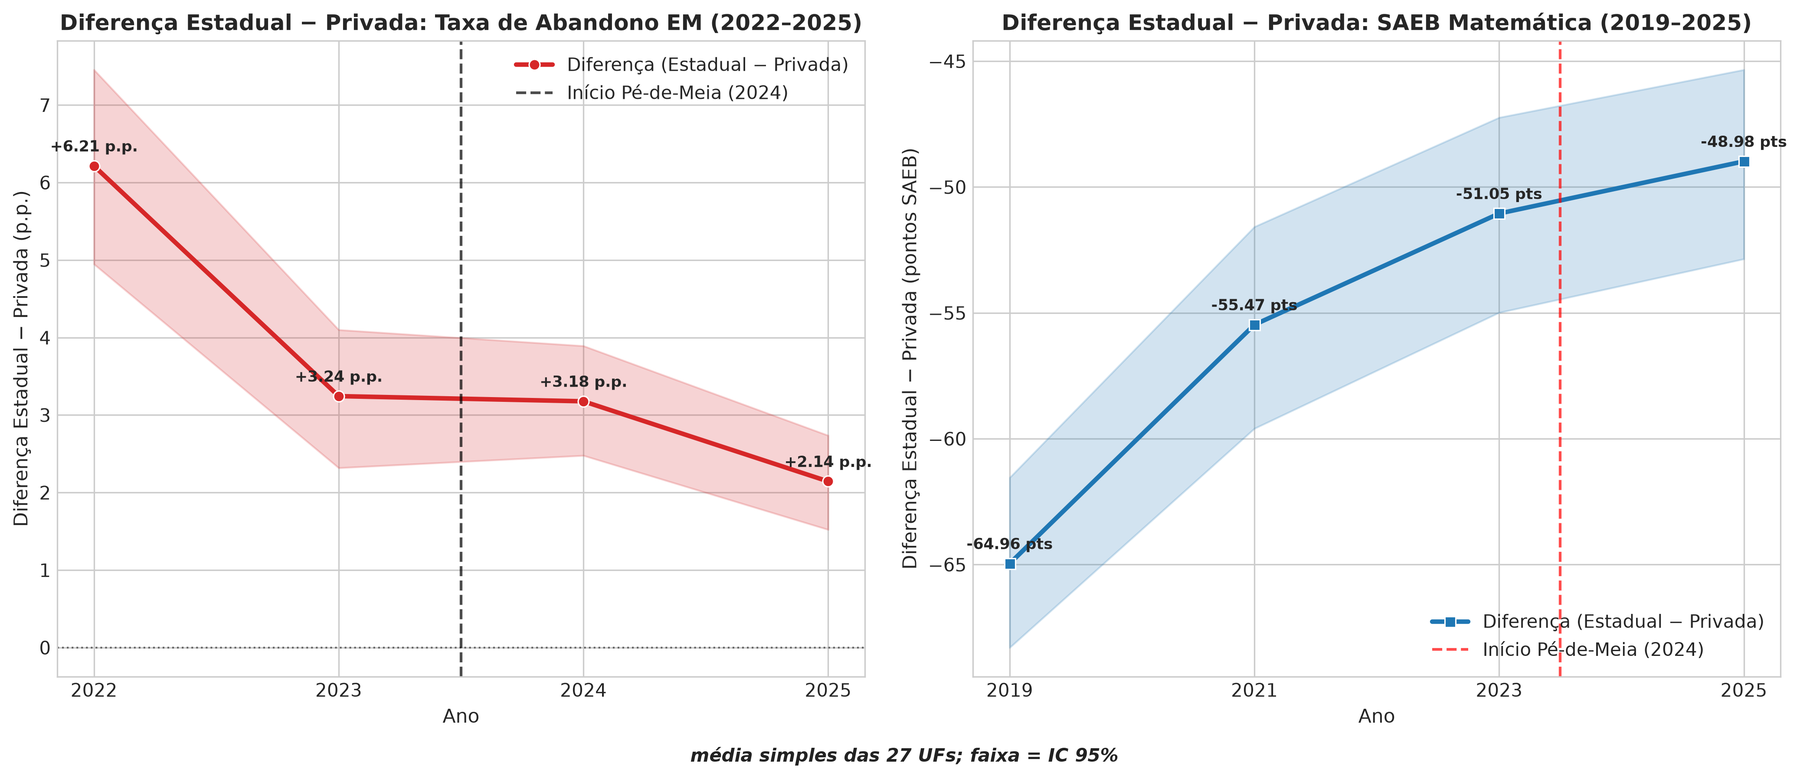
\includegraphics[width=\textwidth]{figuras/grafico_diferenca_estadual_privada}
    \fonte{Elaborada pelo autor (2026) com dados de \citeonline{INEP2026Rendimento} e \citeonline{INEP2026IDEB}. Média simples das 27 UFs; a faixa sombreada representa o intervalo de confiança de 95\%.}
\end{figure}

\subsection{Cenários exploratórios de custo}
\label{subsec_cenarios_custo}

Como as tendências paralelas são rejeitadas, a fração da associação de $-2{,}07$ p.p. no abandono efetivamente atribuível ao programa é desconhecida.
A \autoref{tab_cenarios_custo} apresenta, em caráter estritamente exploratório, o custo nacional por ponto percentual de redução do abandono sob diferentes hipóteses de atribuição, tomando como base o piso do custo do ciclo de 2024 (R\$ 8,71 bilhões).
O cenário de 100\% representa apenas um teto teórico.

\begin{table}[!htb]
    \centering
    \caption{Cenários exploratórios de custo por ponto percentual de redução do abandono (ciclo de 2024, piso)}
    \label{tab_cenarios_custo}
    \small
    \begin{tabular}{ccc}
        \toprule
        \textbf{Atribuição sobre $|\hat{\beta}|$} & \textbf{Redução atribuída (p.p.)} & \textbf{Custo nacional (R\$ bilhões por p.p.)} \\
        \midrule
        100\% (teto teórico) & 2,07 & 4,21 ou mais \\
        50\%                 & 1,03 & 8,43 ou mais \\
        25\%                 & 0,52 & 16,85 ou mais \\
        0\%                  & 0,00 & Não aplicável \\
        \bottomrule
    \end{tabular}
    \fonte{Elaborada pelo autor (2026). Custo do ciclo de 2024 contabilizado até fevereiro de 2025 (R\$ 8.714.892.025,00), interpretado como piso.}
\end{table}

% ------------------------------------------------------------------------------
\section{Discussão}
\label{sec_discussao}

Os resultados apresentam um padrão qualitativamente coerente com a literatura sobre transferências condicionadas: associações expressivas nos indicadores de fluxo escolar (abandono, aprovação e reprovação) e ausência de ganho robusto na proficiência \cite{Fiszbein2009,Glewwe2012}.
A decomposição do IDEB reforça esse padrão, ao mostrar que dois terços do avanço estadual entre 2023 e 2025 decorrem do componente de rendimento.
Esse resultado é consistente com o desenho do Pé-de-Meia, cujos incentivos estão vinculados à matrícula, à frequência e à aprovação, e não ao desempenho em avaliações.

Entretanto, quatro limitações impedem a interpretação causal das estimativas.

\textbf{Violação das tendências paralelas.}
A rejeição da hipótese nula em 11 dos 13 testes de pré-tendência indica que as redes já convergiam antes do programa, impulsionadas pela recuperação pós-pandemia e, possivelmente, pela compressão assintótica da rede privada.
Essa convergência compromete não apenas as janelas longas, mas também a janela imediata, pois não é possível separar empiricamente a continuidade inercial da convergência de uma eventual contribuição do programa \cite{Roth2023}.

\textbf{Multiplicidade de testes.}
Foram realizados 26 testes na especificação principal.
Sob a correção de Bonferroni, nenhum coeficiente da janela imediata permanece significativo, incluindo o IDEB ($p = 0{,}0115$) \cite{Dunn1961}.

\textbf{Agregação ecológica.}
Nem todos os alunos da rede estadual são elegíveis ao programa, de modo que as estimativas correspondem a uma associação em nível de rede, análoga a uma intenção de tratar ecológica.
Inferências sobre o comportamento individual dos beneficiários estão sujeitas à falácia ecológica \cite{Robinson1950}.

\textbf{Políticas concomitantes e variáveis \textit{proxy}.}
No mesmo período, diversas UFs implementaram políticas de busca ativa e de recomposição da aprendizagem que podem afetar os mesmos desfechos.
Além disso, as contagens de beneficiários baseiam-se em \textit{proxies} derivadas das parcelas de pagamento, e o custo do ciclo de 2024 constitui apenas um piso.

Em síntese, os dados agregados disponíveis são compatíveis com uma contribuição do Pé-de-Meia para a melhoria do fluxo escolar, mas não permitem distingui-la da tendência de convergência já em curso.
